%\documentclass{beamer}
%\usetheme{Pittsburgh}
\documentclass{scrartcl}

\usepackage[utf8]{inputenc}
\usepackage{default}
\usepackage[procnames]{listings}
\usepackage{graphicx}
\usepackage{adjustbox}
%\usepackage[toc,page]{appendix}
\usepackage{caption}
\usepackage{hyperref}
\usepackage{color}
%\usepackage{csvsimple}
\usepackage{float}
%\usepackage[T1]{fontenc}



%Bibliogrpahy?
%\usepackage{bibentry}
%\nobibliography*
%\bibentry{ }


%Python
\definecolor{keywords}{RGB}{255,0,90}
\definecolor{comments}{RGB}{0,0,113}
\definecolor{red}{RGB}{160,0,0}
\definecolor{green}{RGB}{0,150,0}
\lstset{language=Python,
    basicstyle=\ttfamily\scriptsize,
    keywordstyle=\color{keywords},
    commentstyle=\color{comments},
    stringstyle=\color{red},
    identifierstyle=\color{green},
    breaklines = true,
    columns=fullflexible,
    %Numbering and tabs
    %numbers=left,
    %numberstyle=\tiny\color{gray},
    %stepnumber=2,
    %numbersep=1em,
    tabsize=4,
    showspaces=false,
    showstringspaces=false}

\begin{document}

\title{Learning and Adaptivity}
\subtitle{Final Report}
\author{
  \href{daiem.ali@smail.inf.h-brs.de}{Ali, Daiem}: \href{https://github.com/daiemna}{github.com/daiemna}\\
  \href{christophe.quignon@smail.inf.h-brs.de}{Quignon, Christophe}:\href{https://github.com/ChrisQuignon}{github.com/ChrisQuignon}
  %Familyname, Name
}
\date{\today}


\maketitle


\begin{abstract}
\textbf{Abstract:}
Heat pumps are a sustainable way to transfer thermal energy into out away from builds to keep a comfortable temperature. But to operate a heating pump is not a trivial task, different building distribute the heat differently and weather with its chaotic nature has a major influence on the temperature flow. With an accurate prediction of the energy consumption, one can increase their efficiency and operating cost.//
In this project, we trained a learning algorithm to predict the energy consumption of one building. Two methods, Gradient Boosting and Random Forests where used and insights from both methods combined. A random forest combined with a sliding window approach lead to the most accurate model with an $R^{2}$ error of 0.89.
\end{abstract}

\section{Data}
\label{sec:data}

The Recogizer GmbH provided a dataset of 4 sensor readings, three weather indicators and an accumulated energy consumption. In 242 days (between July 2014 to February 2015), over 1,300,000 data points where collected.

\paragraph{Weather data:}
The regional weather is from the official recordings of the "Deutsche Wetterdienst" (German weather service) and contains:

\begin{itemize}
\item Temperature in $^\circ C$
\item Relative air humidity in percent
\item Precipitation in mm (1 litre per square meter)
\end{itemize}
\newpage
\paragraph{Sensor data:}
The Measurements from the systems are:

\begin{itemize}
\item Volumetric flow rate in $m^3 / s$
\item Rate of heat flow in watts
\item Supply temperature in $^\circ C$
\item Return temperature $^\circ C$
\end{itemize}

\paragraph{Accumulated data:}
The energy in watt hours, calculated per day.

\section{Analysis}
\label{sec:analysis}
\subsection{Seasonal decomposition}
Our data has a seasonal trend which is shown in the figure \ref{fig:season_outside_temperature}. In the figure the seasonal trend of one whole week outside temperature is shown. We can see the repeating peaks for every day. For this reason we introduced the day of the year(DOY) as a feature which allows the learning algorithm to include the seasonal effects. The effect of introducing DOY is shown in figure \ref{fig:RandomForestRegressor_day_error_without_some_params_DOY}

\begin{figure}[H]
  \center
  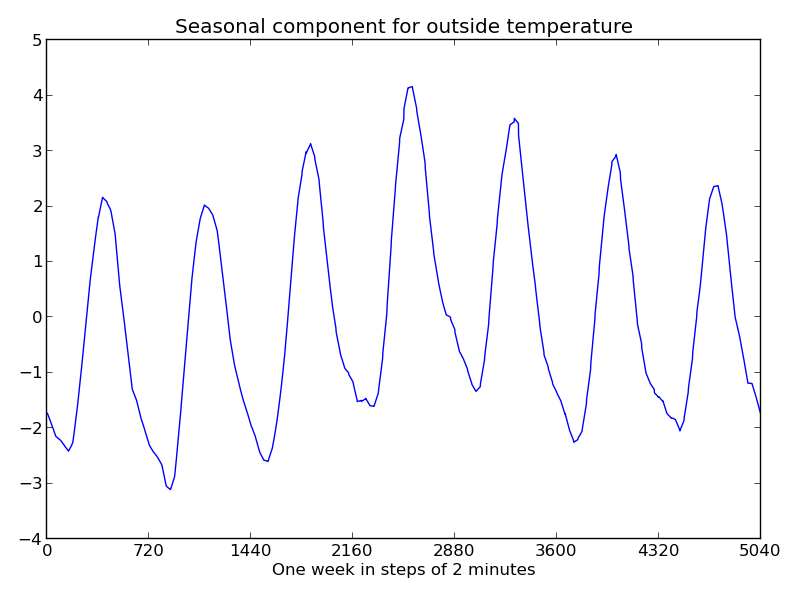
\includegraphics[width=0.6\linewidth]{img/season-outside_temperature.png}
  \caption{Seasonal (weekly) decomposition of the datasets.}
  \label{fig:season_outside_temperature}
\end{figure}


\begin{figure}[H]
  \center
  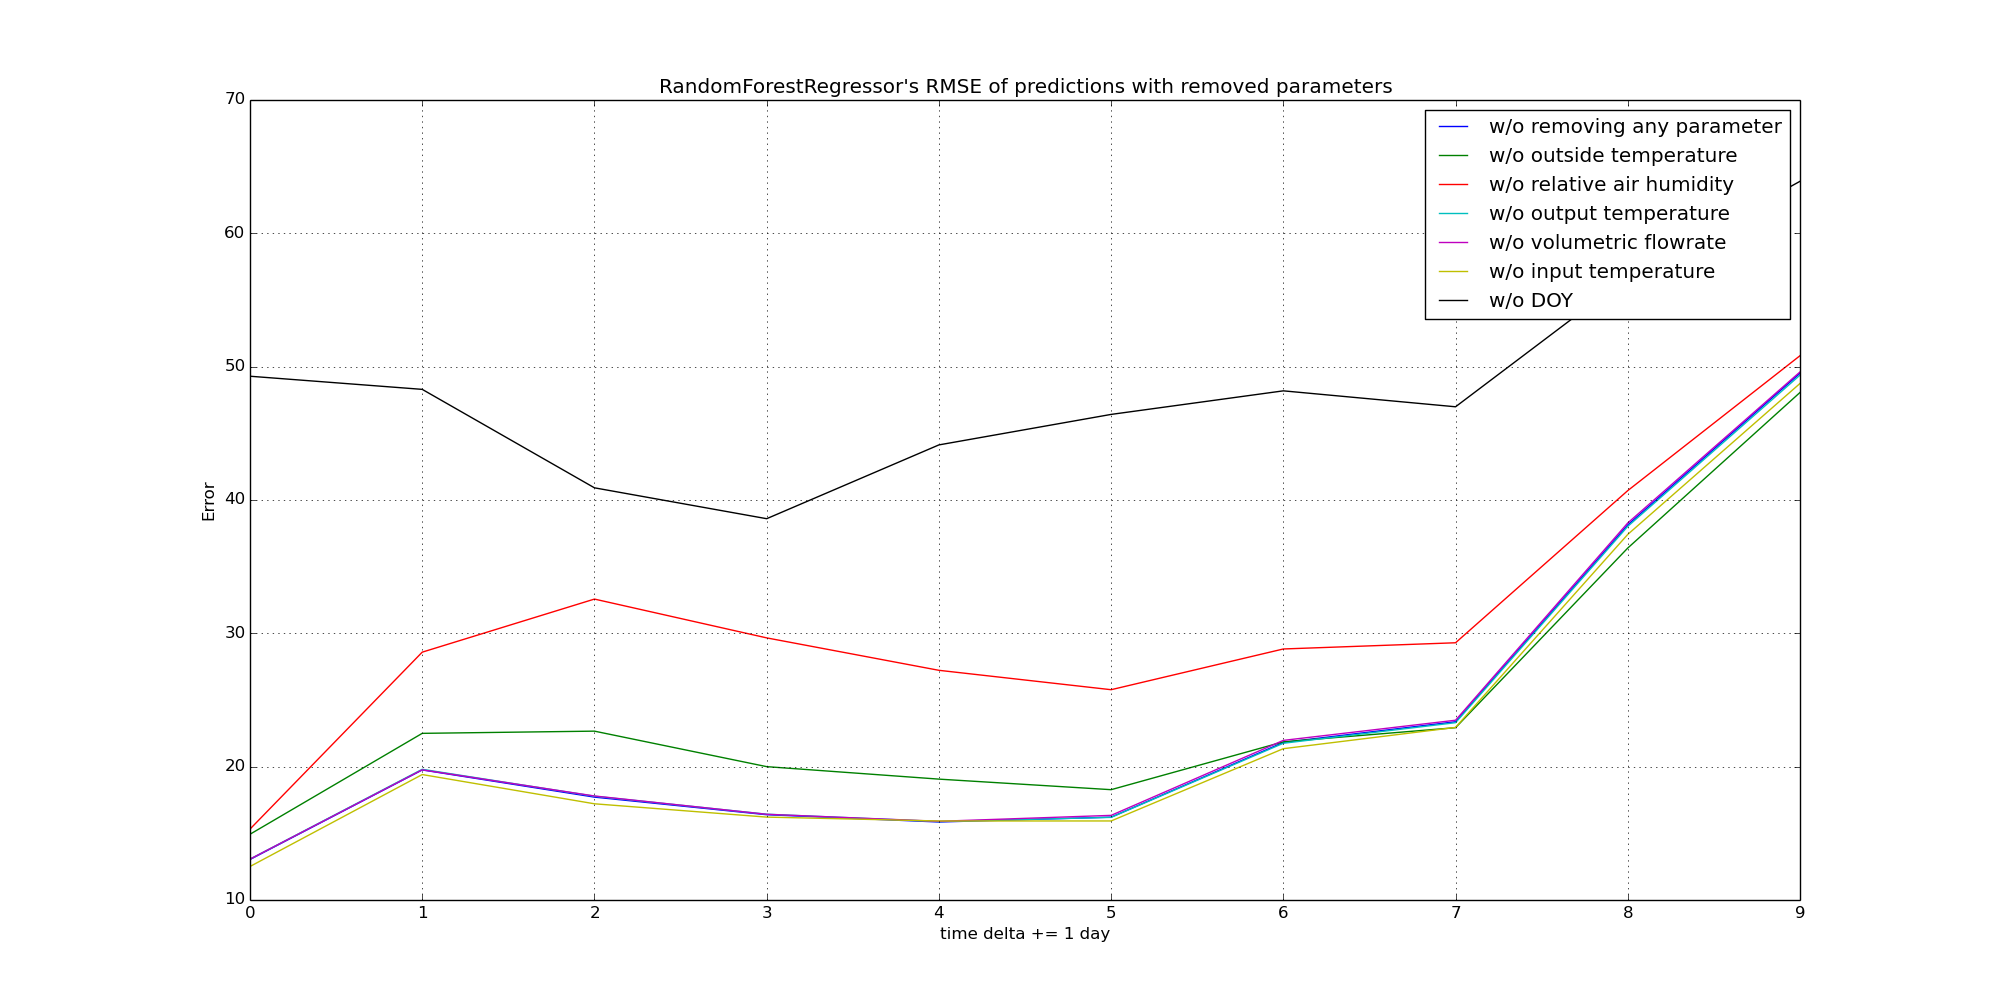
\includegraphics[width=1\linewidth]{img/RandomForestRegressor_day_error_without_some_params_DOY.png}
  \caption{Random Forest with Day of the Year information}
  \label{fig:RandomForestRegressor_day_error_without_some_params_DOY}
\end{figure}


\subsection{Exclusion of precipitation}	
During analysis we assessed the importance of features. To study this we removed each feature and plotted the Root Mean Squared Error (RMSE) of the predictions. It can be seen form the figure \ref{fig:RandomForestRegressor_day_error_without_some_params} and figure \ref{fig:RandomForestRegressor_day_error_without_precipation}, that there is little to no effect on RMSE without precipitation.


\begin{figure}[H]
  \center
  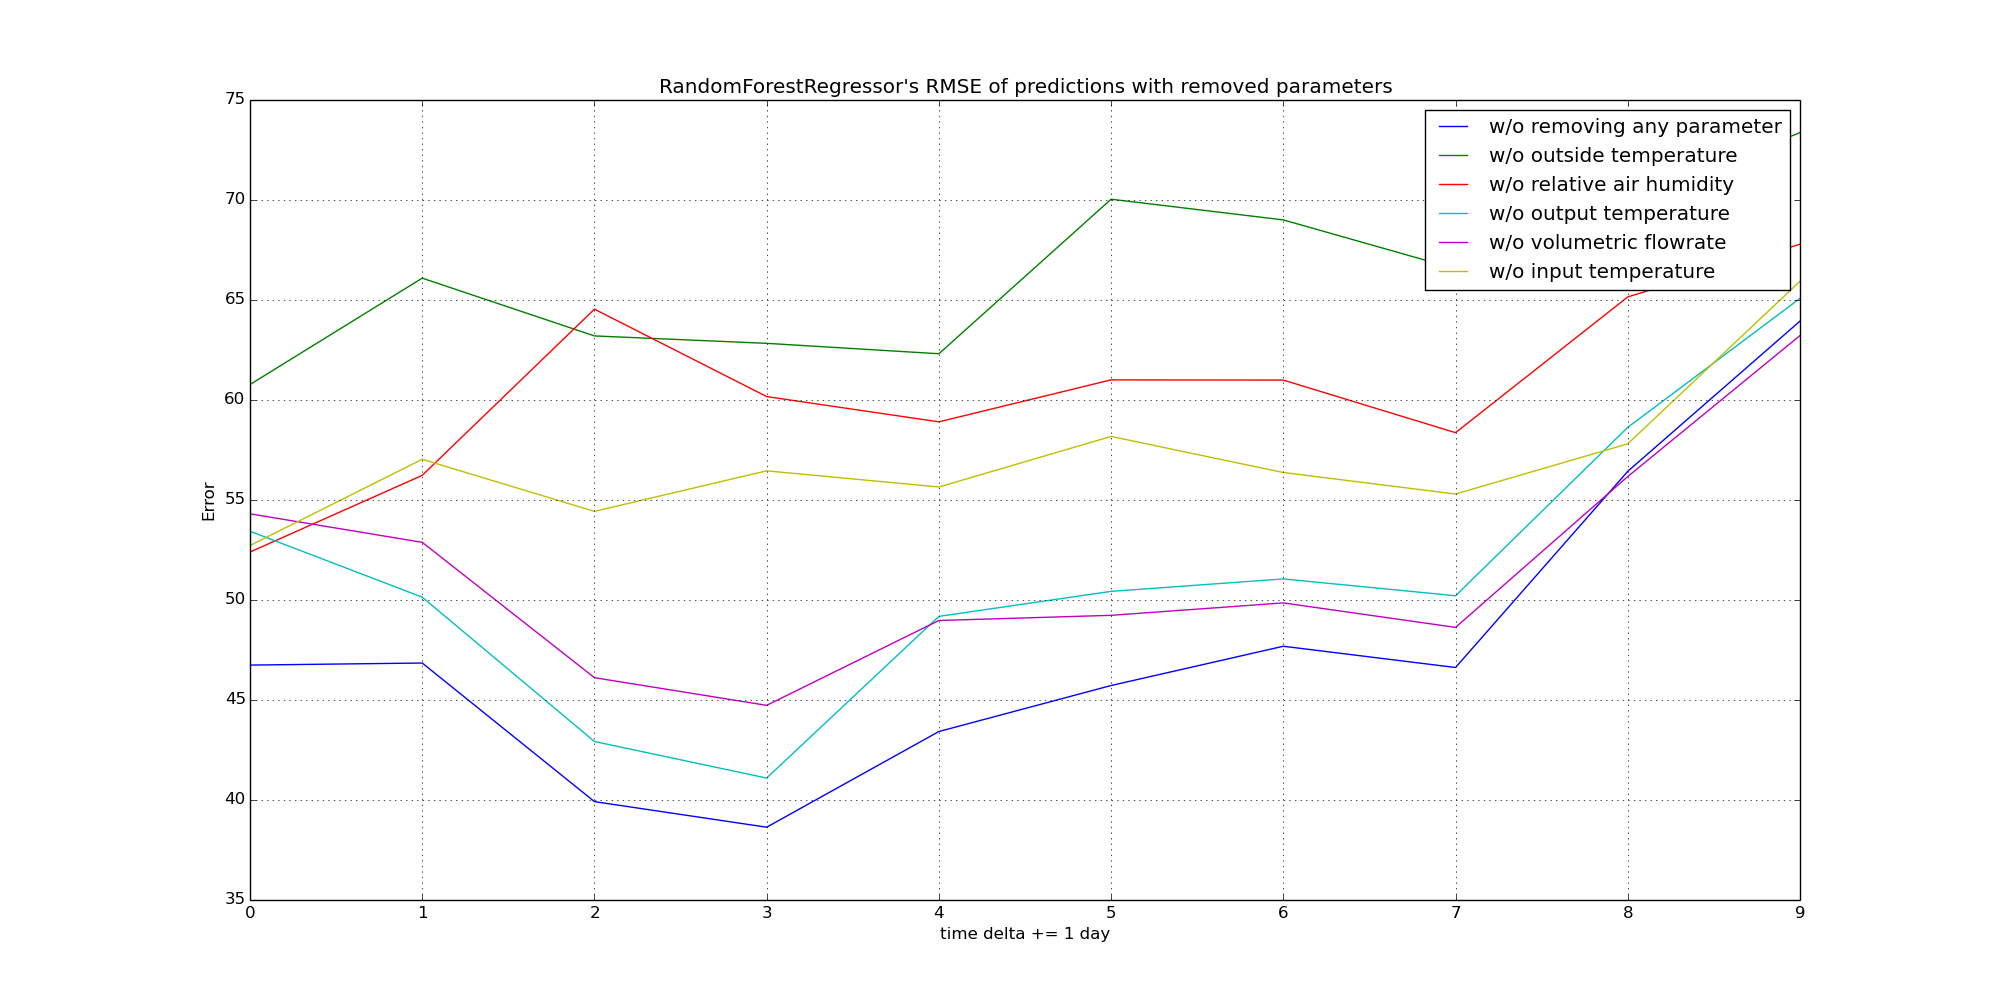
\includegraphics[width=1\linewidth]{img/RandomForestRegressor_day_error_without_some_params.png}
  \caption{Random Forest with effect of removing each parameter}
  \label{fig:RandomForestRegressor_day_error_without_some_params}
\end{figure}


\begin{figure}[H]
  \center
  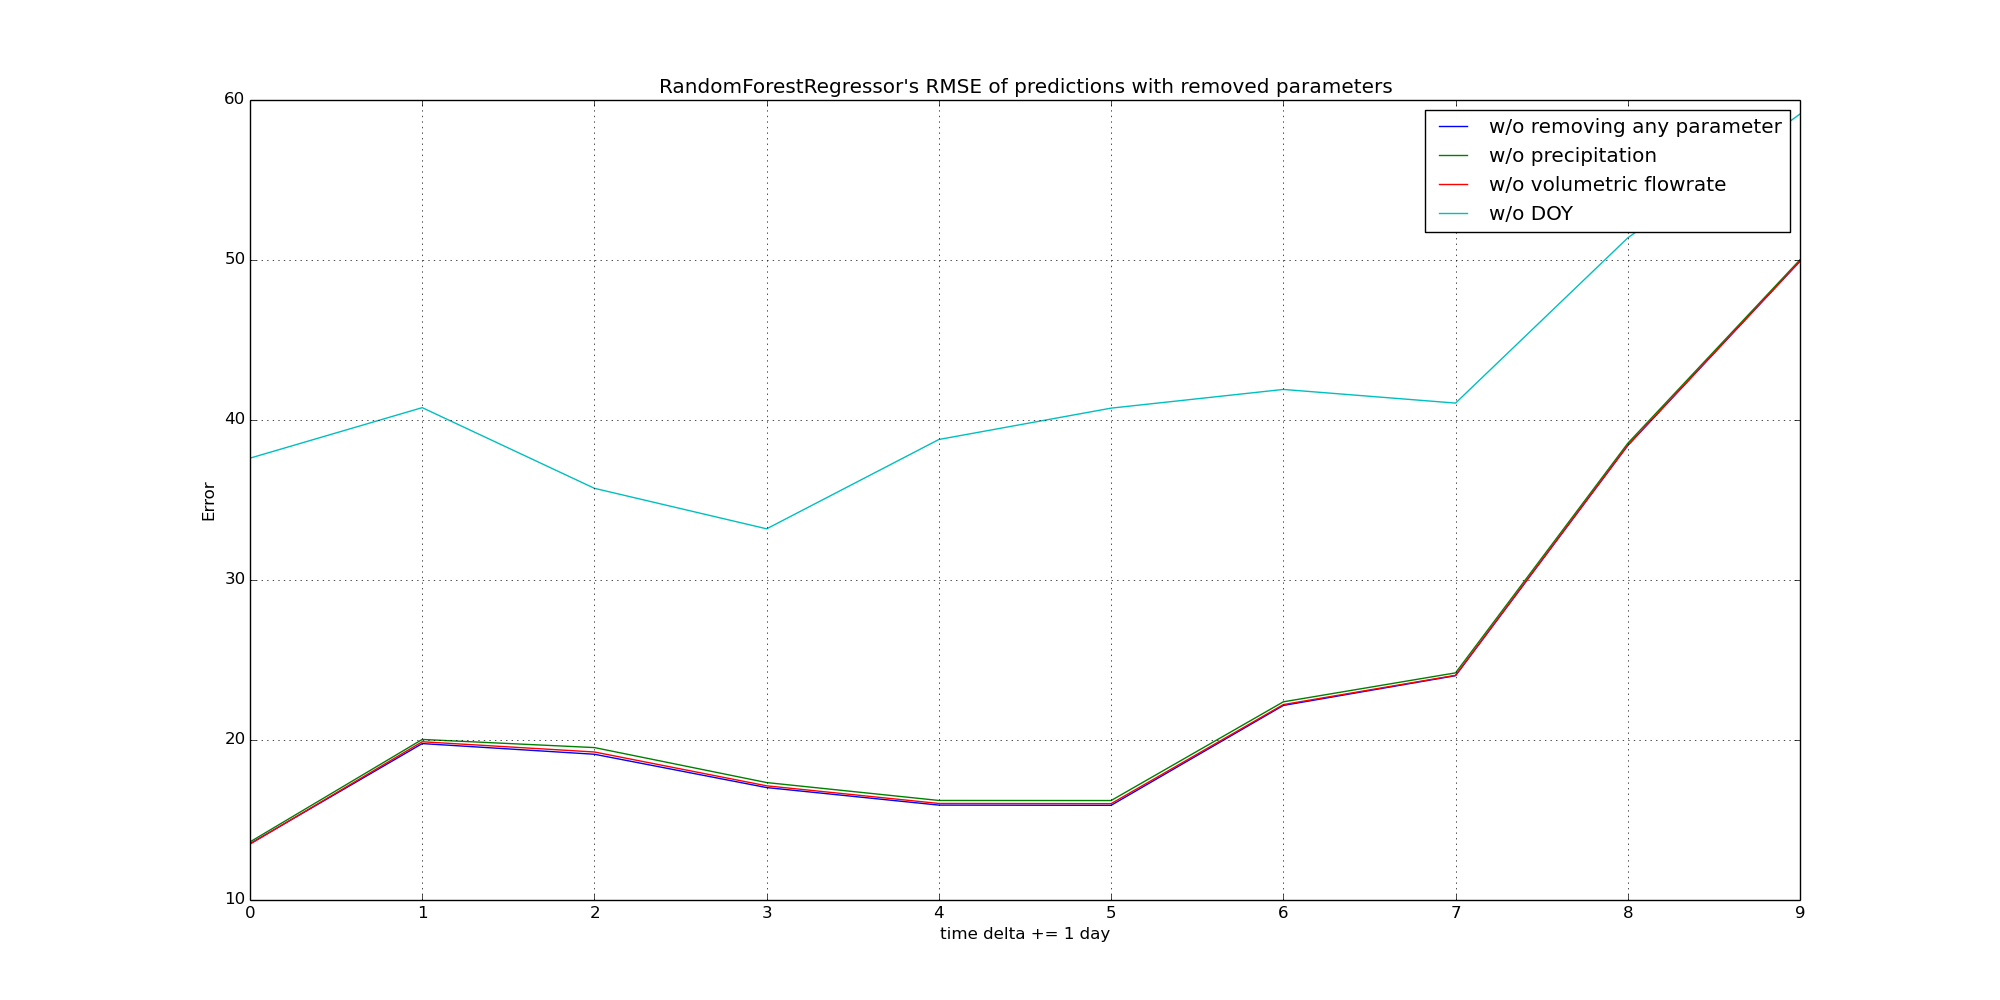
\includegraphics[width=1\linewidth]{img/RandomForestRegressor_day_error_without_precipation.png}
  \caption{Random Forest without Precipitation}
  \label{fig:RandomForestRegressor_day_error_without_precipation}
\end{figure}

\section{Methods}
\label{sec:methods}
To find an optimal prediction, we analysed two methods: For the gradient boosting we took a standard implementation and looked for optimal parameter, where for the time shifting window approach we focussed on the preprocessing of the data.

\subsection{Sliding Window}
As suggested in \cite{vafaeipour2014application} the sliding window approach was used to learn how to predict. In this approach the time series is split into windows or frames of input and output. Unlike in regression learning, those windows are shifted. Thus the learning algorithm does not learn the relation of the features at the same time, but their relation in the future. With this approach, it is possible to include all features as an input and select few of them as an output. This can be enhanced further by including predictable features into the input. These three methods are depicted in Figure \ref{fig:slidingwindow}.
\begin{figure}[H]
  \center
  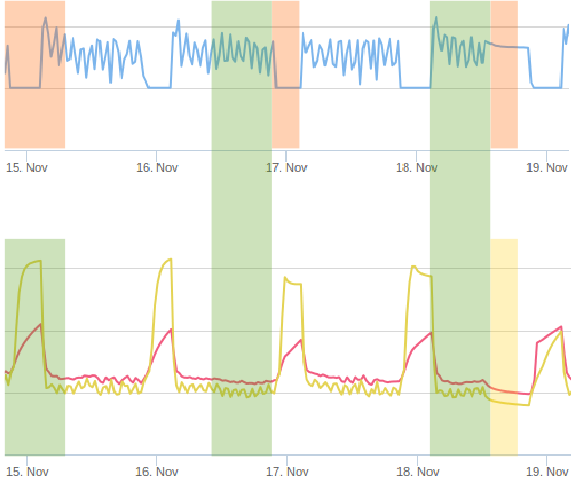
\includegraphics[width=0.6\linewidth]{img/regpred.png}
  \caption{Input(green) and output(red) frames for regression(left), prediction(middle) and enhanced prediction(right).}
  \label{fig:correlation}
\end{figure}

\subsection{Gradient Boosting}
Gradient Boosting is a performant way to regress functions for prediction. This quick learning time enabled us to run several sets of features and  plot the increase in error as seen in figure \ref{fig:GradientBoostingRegressor_day_error_without_some_params}. 

\begin{figure}[H]
  \center
  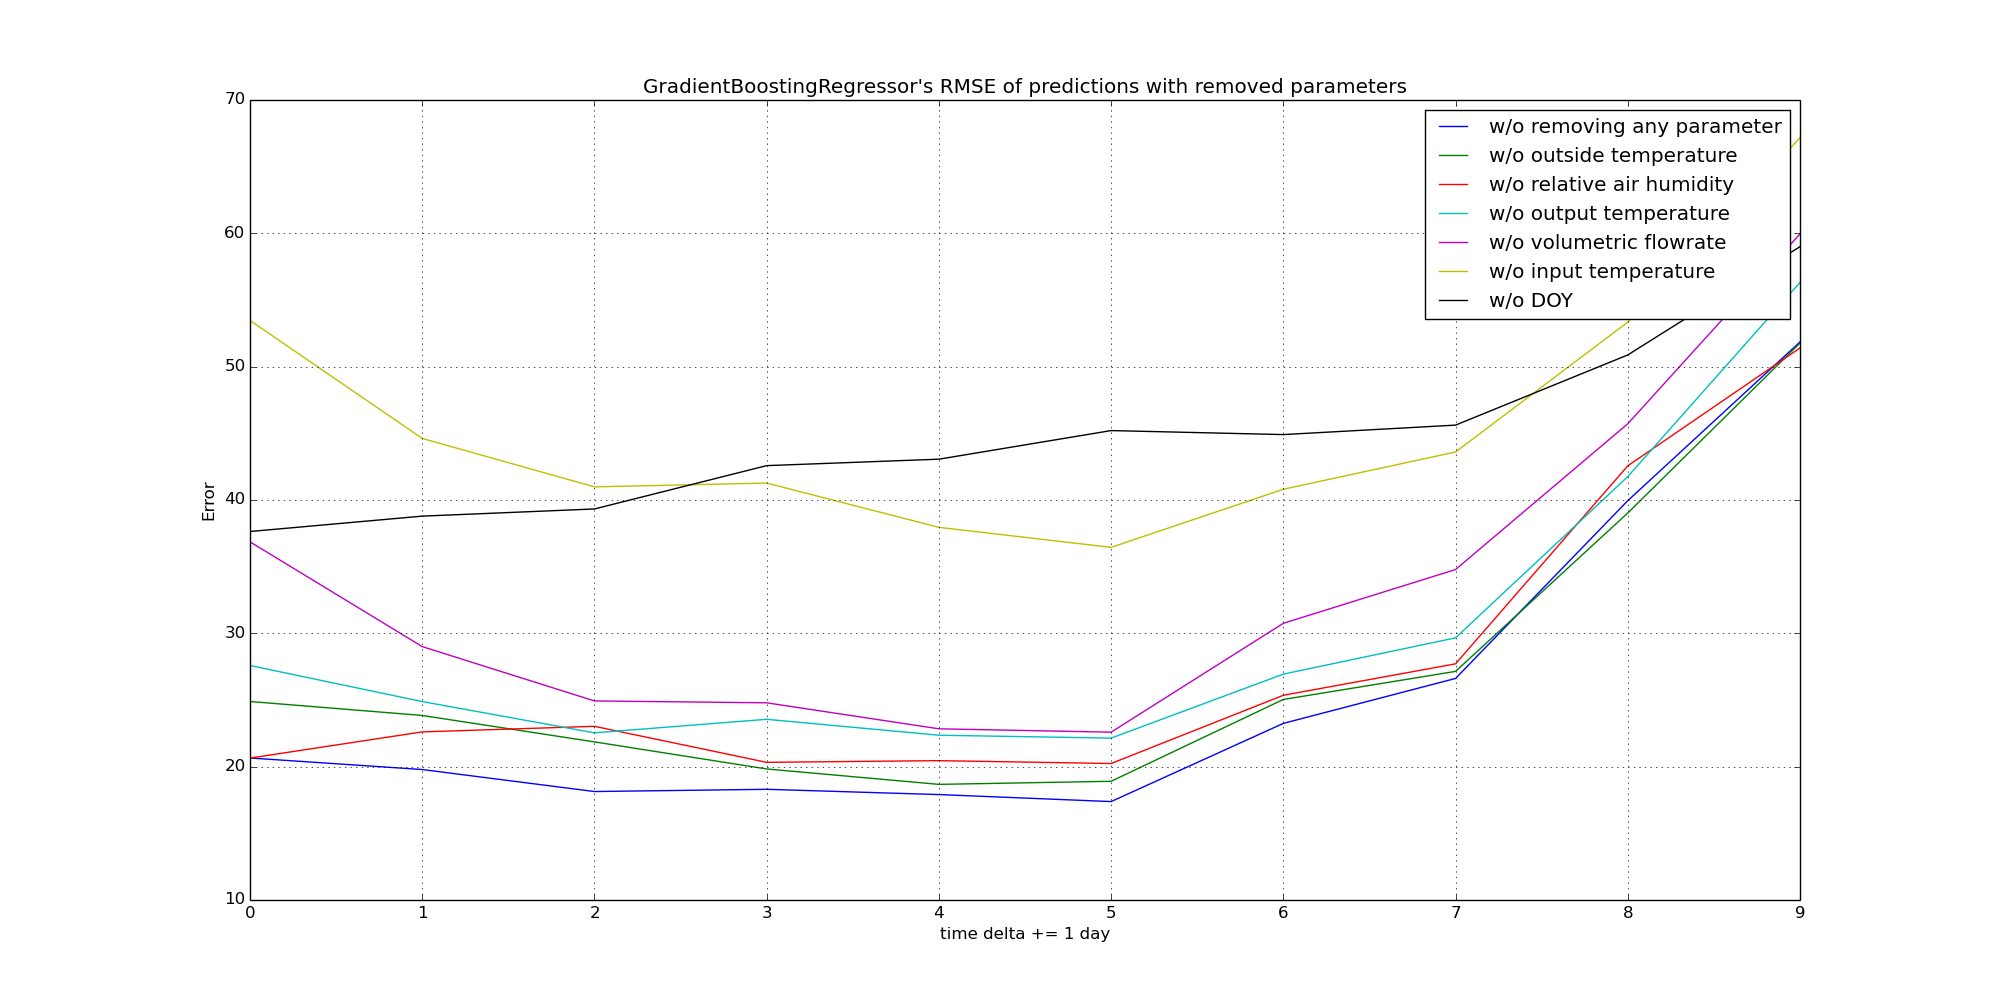
\includegraphics[width=1\linewidth]{img/GradientBoostingRegressor_day_error_without_some_params.png}
  \caption{Error over time with the Gradient Boosting regression on several feature sets.}
  \label{fig:GradientBoostingRegressor_day_error_without_some_params}
\end{figure}
\newpage
\section{Conclusion}
\label{sec:conclusion}
The best $R^{2}$ score (0.89) of all runs was learned by a Random Forest combined with a sliding window approach, without precipitation and with the day of the year. It can be seen in the figure \ref{fig:predict-energy} that random forest is able to predict the energy successfully based on averaged energy information.\\
The gradient boosting was a good help in terms of prediction time, we analysed different subsets of our data on gradient boosting and then applied them on the random forests.
\begin{figure}[H]
  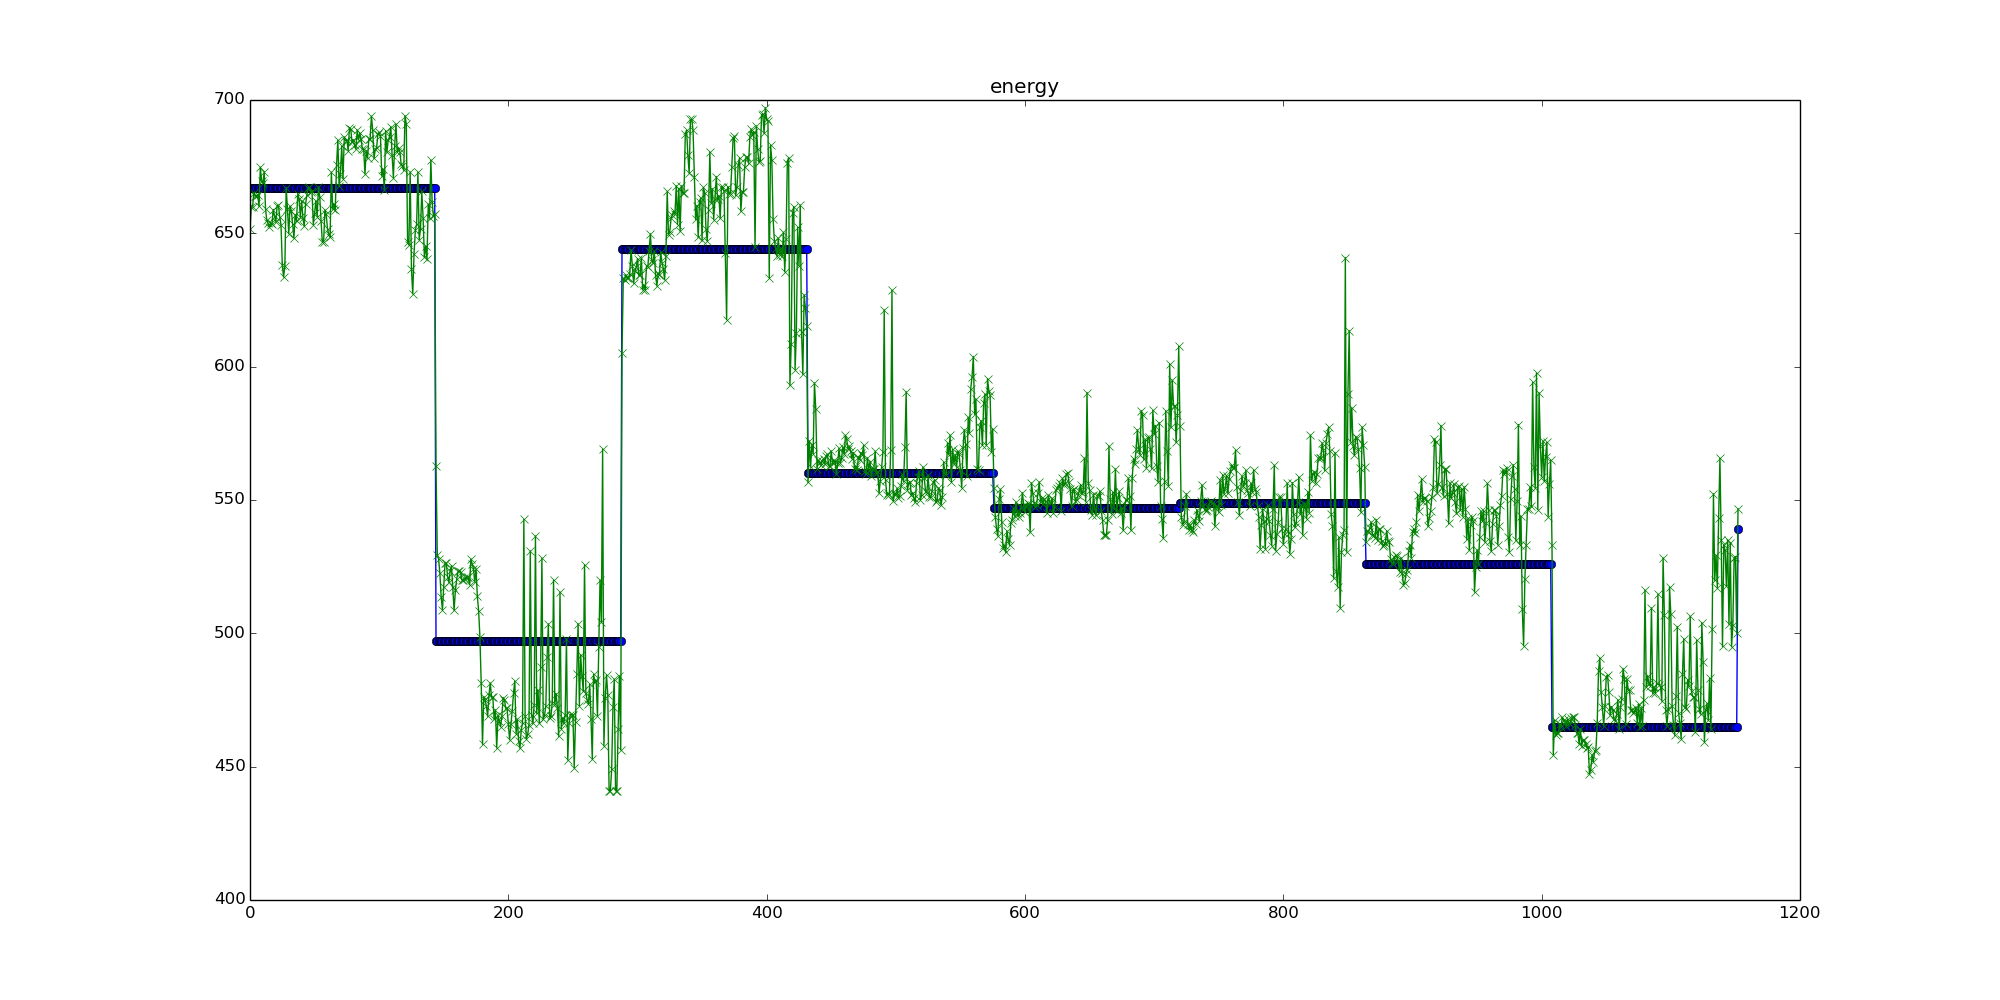
\includegraphics[width=0.8\linewidth]{img/predict-energy--0p890.png}
  \caption{Prediction (green) of the energy(blue) using the sliding window approach.}
  \label{fig:predict-energy}
\end{figure}
It is evident that the random forest is capable of predicting the energy consumption for 5 days in advance. In our study we tweaked the input with the sliding window approach and analysed the data with test runs on gradient boosting. The choice of random forest can be justified form the comparison with gradient boosting. In addition, the rules of the single random trees can be interpreted by humans and thus checked by experts. We expect that the performance can be further improved by including the weather forecast, but this will make the prediction greatly depended on the accuracy of the weather forecast. Thus also is likely to make the performance of the regression deteriorate faster.

%BIBLIOGRPAHY
\bibliographystyle{plain}%amsalpha
\bibliography{bib.bib}
%\bibentry{}

%\begin{appendix}
%\section{}

%\end{appendix}


%COPY AND PASTE FROM HERE

%\begin{enumerate}
% \item
%\end{enumerate}

%\href{link}{text}

%\begin[Language=Python]{lstlisting}
%#PYTHON CODE HERE
%\end{lstlisting}

%\lstinputlisting[language=Python]{	}

%\csvautotabular[separator=semicolon]{data.csv}


%\begin{figure}[H]
%  \centering
%  \includegraphics[width=0.5\linewidth]{../img/	}
%  %\caption{}
%  %\label{fig:}
%\end{figure}
%PUT UNITS ON THE FIGURES

\end{document}
